\documentclass[9pt]{beamer}

\usetheme{metropolis}
%\usefonttheme[onlymath]{serif}
\usefonttheme[onlymath]{serif}

\usepackage{presentation}

\newcommand{\pp}{p\para}
\newcommand{\qp}{q\para}
\newcommand{\rp}{r\para}

\usepackage{fontspec}
\setsansfont{IBM Plex Serif}

\title{Interpretable Latent Variable Models for Graphs}
\subtitle{UGP Presentation}
\date{24th November, 2018}
\author{Gurpreet Singh}
\institute{Indian Institute of Technology, Kanpur}

\begin{document}
\frame{\titlepage}

\section{Background}

\subsection{Black Box Variational Inference}
\begin{frame}{BBVI - Overview}
	In Variational Inference, the optimization objective is given by the ELBO
	\begin{align*}
		\logp{\qp{\vx}} \ge \elbo{\vx, \vphi} = \E[\vz \sim q(\vz \spipe \vx, \vphi)]{\logp{p(\vx, \vz)} - \logp{q(\vz \pipe \vx, \vphi)}}
	\end{align*}

	Black Box Variational Inference is based on stochastic optimization of the variational objective
	\begin{align*}
		\nabla \elbo{\vx, \vphi} &= \E[q(\vz \spipe \vx, \vphi)]{\nabla_\vphi \logp{q(\vz \pipe \vx, \phi)} \para{\logp{p(\vx, \vz)} - \logp{q(\vz \pipe \vx, \vphi)}}}
	\end{align*}

	The above term is known as the Score Function.

\end{frame}

\begin{frame}{BBVI - Reparameterization}
	If we can find a reparametrization $\vepsilon = f^{-1}(\vz, \vphi)$ such that $\vepsilon$ is independent of $\vphi$, then
	\begin{align*}
		\nabla \elbo{\vx, \vphi} = \E[q(\vepsilon)]{\nabla_\vz \brac{\logp{p(\vx, \vz)} - \logp{q(\vz \pipe \vx, \vphi)}}_{\vz = f(\vepsilon, \vphi)} \nabla_{\vphi} f(\vepsilon, \vphi)}
	\end{align*}

	If $\vz$ is discrete $p(\vz)$ is a p.m.f. and therefore, the derivatives no longer exist. Hence, reparameterization is \bt{not} possible
\end{frame}

\begin{frame}{Discrete Latent Variables}
	Some methods to train discrete latent variable models -
	\begin{enumerate}
		\item Marginalize all discrete latent variables
		\item Using local expectation gradients, and reparametrization and marginalization % Essentially based on the idea that the value of a parameter depends only on a few values, however requires multiple function evaluations per gradient
		\item Relaxed computation of discrete densities (straight through approach)
		\item Smooth relaxations for discrete variables (e.g. Concrete Distribution)
		\item Using the Score Function approach with variance reduction using control variates/non-uniform sampling.
	\end{enumerate}
\end{frame}

\section{Gumbel-Softmax Trick}
\begin{frame}{The Concrete Distribution}
	Sampling from a categorical distribution: Sample U from a $\brac{0, 1}$ uniform distribution, then reparameterize as
	\begin{align*}
		\sC = \argmax{k \in \brac{K}} \logp{\alpha_k} - \log{-\log{\sU_k}}
	\end{align*}

	A softmax version of this can be used as smooth relaxations
	\begin{align*}
		\sZ_k = \frac{\texp{\para{\logp{\alpha_k} + G_k} / \tau}}{\sum_{k' = 1}^K \texp{\para{\logp{\alpha_{k'}} + G_{k'}} / \tau}}
	\end{align*}
	where $\tau$ is the \bt{temperature} parameter.
\end{frame}

\section{Discrete Variational Autoencoders}
\begin{frame}{Discrete Variational Autoencoders}
	Gumbel-Softmax trick only works for factorial priors. Discrete Variational Autoencoders are models which work with more expressive priors, the (Restricted) Boltzmann Machine priors.

	\bt{Boltzmann Machine Prior}
	\begin{align*}
		\qp{\vz} &= \frac{\exp{-E(\vz)}}{Z_\theta}, \hspace{0.5cm} \mt{where}\\
		E(\vz) &= \trans{\vz} \vb + \trans{\vz} \sW \vz
	\end{align*}

	\bt{Restricted Boltzmann Machine Prior}
	\begin{align*}
		E(\vz) &= \trans{\vz_1} \vb_1 + \trans{\vz_2} \vb_2 + \trans{\vz_1} \sW \vz_2
	\end{align*}
\end{frame}

\begin{frame}{Discrete Variational Autoencoders}
	\begin{figure}[htpb]
		\begin{subfigure}[b]{0.49\textwidth}
			\centering
			\resizebox{0.7\textwidth}{!}{%
				\begin{tikzpicture}[->, >=stealth', shorten >=1pt, auto, node distance=1.8cm, semithick, scale=\textwidth/15.2cm]
					\node[state]	(x)				 	{$\vx$};
					\node[state]	(z2) [below of=x]	{$\vz_2$};
					\node[state]	(z1) [left of=z2]	{$\vz_1$};
					\node[state]	(z3) [right of=z2]	{$\vz_3$};
					\node[state]	(c1) [below of=z1]	{$\vzeta_1$};
					\node[state]	(c2) [below of=z2]	{$\vzeta_2$};
					\node[state]	(c3) [below of=z3]	{$\vzeta_3$};

					\path	(x)		edge	node	{}	(z1)
					edge	node	{}	(z2)
					edge	node	{}	(z3)
					(z1)	edge	node	{}	(c1)
					(z2)	edge	node	{}	(c2)
					(z3)	edge	node	{}	(c3);
				\end{tikzpicture}
			}
			\caption{Posterior Network ($\qp{\vzeta, \vz \pipe \vx}$)}
			\label{fig:dvae-network:posterior}
		\end{subfigure}
		\begin{subfigure}[b]{0.49\textwidth}
			\centering
			\resizebox{0.7\textwidth}{!}{%
				\begin{tikzpicture}[->, >=stealth', shorten >=1pt, auto, node distance=1.8cm, semithick]
					\node[state]	(z2)			 	{$\vz_2$};
					\node[state]	(z3) [right of=z2]	{$\vz_3$};
					\node[state]	(z1) [left of=z2]	{$\vz_1$};
					\node[state]	(c1) [below of=z1]	{$\vzeta_1$};
					\node[state]	(c2) [below of=z2]	{$\vzeta_2$};
					\node[state]	(c3) [below of=z3]	{$\vzeta_3$};
					\node[state]	(x)  [below of=c2]	{$\vx$};

					\draw[-] ;

					\path	(z1)	edge						node	{}	(c1)
									edge [-]					node	{}	(z2)
									edge [-, out=30, in=150]	node	{}	(z3)
							(z2)	edge						node	{}	(c2)
									edge [-]					node	{}	(z3)
							(z3)	edge						node	{}	(c3)
							(c1)	edge						node	{}	(x)
							(c2)	edge						node	{}	(x)
							(c3)	edge						node	{}	(x);
				\end{tikzpicture}
			}
			\caption{Prior Network ($\pp{\vzeta, \vz}$)}
			\label{fig:dvae-network:prior}
		\end{subfigure}
		\caption{Graphical Models of the approximating posterior (a) and the prior (b)}
		\label{fig:dvae-network}
	\end{figure}
\end{frame}

\begin{frame}{Discrete Variational Autoencoders}
	The prior $p(\vzeta, \vz \pipe \vtheta)$ is suitably written as
	\begin{align*}
		\pp{\vzeta, \vz \pipe \vtheta}	&= r\para{\vzeta \pipe \vz} \cdot \pp{\vz \pipe \vtheta}, \hspace{1cm} \mt{where} \\
		r\para{\vzeta \pipe \vz}			&= \prod_i r\para{\zeta_i \pipe z_i}
	\end{align*}
	The posterior is correspondingly augmented as
	\begin{align*}
		\qp{\vzeta, \vz \pipe \vx, \vphi} = \rp{\vzeta \pipe \vz} \cdot \qp{\vz \pipe \vx, \vphi}
	\end{align*}
	The log-likelihood is assumed to have the following property
	\begin{align*}
		\qp{\vx \pipe \vz, \vzeta, \vtheta} = \qp{\vx \pipe \vzeta, \vtheta}
	\end{align*}
\end{frame}

\begin{frame}{DVAEs - Computing the Gradients}
	In the VAE framework, we decomompose the ELBO as
	\begin{align*}
		\elbo{\vz, \vphi} = \underbrace{- \kld{\qp{\vzeta, \vz \pipe \vx, \vphi}}{\pp{\vzeta, \vz \pipe \vtheta}}}_\text{KL Term} + \underbrace{\E[q(\vzeta, \vz \spipe \vx, \vphi)]{p(\vx \pipe \vzeta, \vtheta)}}_\text{Autoencoding Term}
	\end{align*}
	The gradients of the KL term are given as
	\begin{align*}
		\nabla \kld{q}{p} &= \underbrace{\E[q(\vz \spipe \vx, \vphi)]{\nabla E_\vtheta(\vz)} - \E[p(\vz \spipe \vtheta)]{\nabla E_\vtheta(\vz)}}_\text{Gradients for Prior Parameters} \ + \\
		& \underbrace{\sum_{i} \sum_{z_i} \qp{z_i \pipe \vx, \vphi} \logp{\qp{z_i \pipe \vx, \vphi}} + \nabla E_\vtheta\para{\E[q(\vz \spipe \vx, \vphi)]{\vz}}}_\text{Gradients for Posterior Parameters}
	\end{align*}
\end{frame}

\begin{frame}{DVAE - Spike-and-Exponential Smoothing}
	$\rp{\zeta_i \pipe z_i}$ for spike-and-exp transformation is given as
	\begin{align*}
		\rp{\zeta_i \pipe z_i = 0}	&= \delta_{0}(\zeta_i) \\
		\rp{\zeta_i \pipe z_i = 1}	&= \frac{\beta \exp{\beta \zeta}}{\exp{\beta} - 1},	\ \mt{if} \zeta_i \in \brac{0, 1} \mt{else,} 0
	\end{align*}
	The inverse CDF for the same is given as
	\begin{align*}
		\zeta_i = F_{\qp{\zeta_i \spipe \vx, \vphi}}^{-1}(\rho_i)	= \max\set{\frac{1}{\beta} \cdot \logp{\brac{\para{\frac{\rho_i + q_i - 1}{q_i}} \cdot \para{\exp{\beta} - 1}} + 1}, 0}
	\end{align*}
	where $\rho_i \in \para{0, 1}$ is sampled from a uniform distribution (from 0 to 1), and $q_i$ is the short-hand notation for $\qp{z_i \pipe \vx, \vphi}$.

\end{frame}

\begin{frame}{DVAE++ - Exp-and-Exp smoothing}
		$\rp{\zeta_i \pipe z_i}$ for exp-and-exp transformation, similar to the spike-and-exp case, is given as
		\begin{align*}
			\rp{\zeta_i \pipe z_i = 0}	&= \frac{\beta \exp{\beta (1 - \zeta)}}{\exp{\beta} - 1},	\ \mt{if} \zeta_i \in \brac{0, 1} \mt{else,} 0 \\
			\rp{\zeta_i \pipe z_i = 0}	&= \frac{\beta \exp{\beta \zeta}}{\exp{\beta} - 1},	\ \mt{if} \zeta_i \in \brac{0, 1} \mt{else,} 0
		\end{align*}
		The inverse CDF in this case is given (details in the original paper) as
		\begin{align*}
			\zeta_i = F_{\qp{\zeta_i \spipe \vx, \vphi}}^{-1}(\rho_i)	= - \frac{1}{\beta} \cdot \logp{\frac{-b + \sqrt{b^2 - 4ac}}2}
		\end{align*}
		where $\rho \in \para{0, 1}$ is sampled from a uniform distribution (from 0 to 1), and $b = \brac{\rho + \exp{-\beta}(q_i - \rho)} / (1 - q_i) - 1$, $c = \para{q_i \exp{- \beta}}/(1 - q_i)$, and $q_i$ is the short-hand notation for $\qp{z_i \pipe \vx, \vphi}$.
\end{frame}

\section{The Gumbolt Trick}
\begin{frame}{Gumbolt - Relaxed ELBO}
	The posterior and the prior for the smoothing variables are given as
	\begin{align*}
		\pp{\vzeta \pipe \vtheta} &= \frac{\exp{-E_{\vtheta}(\vzeta)}}{\widetilde{Z}_{\vtheta}}, \ \mt{where} \widetilde{Z}_\vtheta = \int_\vzeta \exp{E_\vtheta(\vzeta)} \id \vzeta \\
		\qp{\vzeta \pipe \vx, \vphi} &= \prod_{i} \zeta_i q_i + (1 - \zeta_i)(1 - q_i)
	\end{align*}
	The alternate ELBO, therefore, is given as
	\begin{align*}
		\widetilde{\cL}\para{\vx, \vphi} = &\E[\qp{\vzeta \spipe \vx, \vphi}]{\logp{\pp{\vx \pipe \vzeta, \vtheta}} - \logp{\qp{\vzeta \pipe \vx, \vphi}} - E_\vtheta(\vzeta)} - \logp{\widetilde{Z}_{\vtheta}}
	\end{align*}
\end{frame}

\begin{frame}{Gumbolt - Relaxed ELBO}
	Relaxed ELBO is given as
	\begin{align*}
		\breve{\cL}\para{\vx, \vphi} = &\E[\qp{\vzeta \spipe \vx, \vphi}]{\logp{\pp{\vx \pipe \vzeta, \vtheta}} - \logp{\qp{\vzeta \pipe \vx, \vphi}} - E_\vtheta(\vzeta)} - \logp{Z_{\vtheta}}
	\end{align*}
	where, we have
	\begin{align*}
		\logp{\pp{\vx \pipe \vtheta}} \ge \widetilde{\cL}\para{\vx, \vphi} \ge \breve{\cL}\para{\vx, \vphi}
	\end{align*}

	Also, as $\tau \ra 0$, $\breve{\cL} \ra \widetilde{\cL}$
\end{frame}

\begin{frame}{Gumbolt - Regeneration}
	\begin{figure}[htpb]
		\centering
		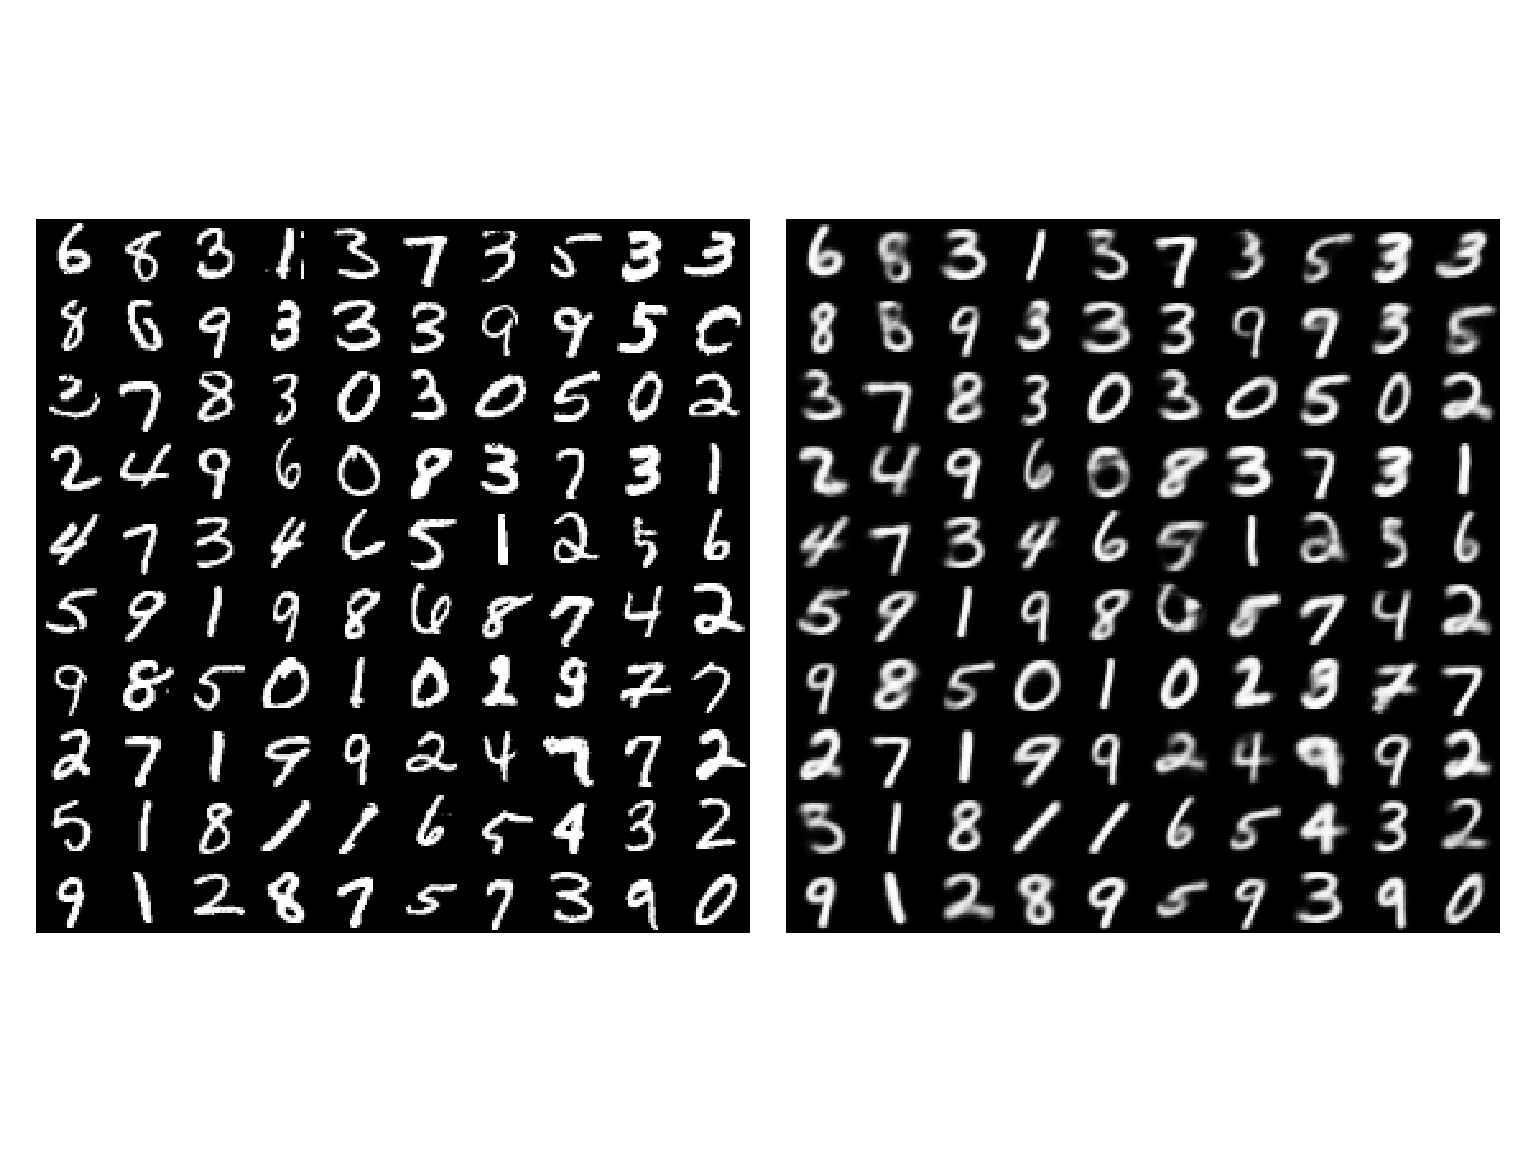
\includegraphics[height=200px]{includes/plots/gumbolt-vae/mnist/regenerated.png}
		\caption{Regerenation Plot for Gumbolt-Vae}
	\end{figure}
\end{frame}

\begin{frame}{Gumbolt - Sampling}
	\begin{figure}[htpb]
		\centering
		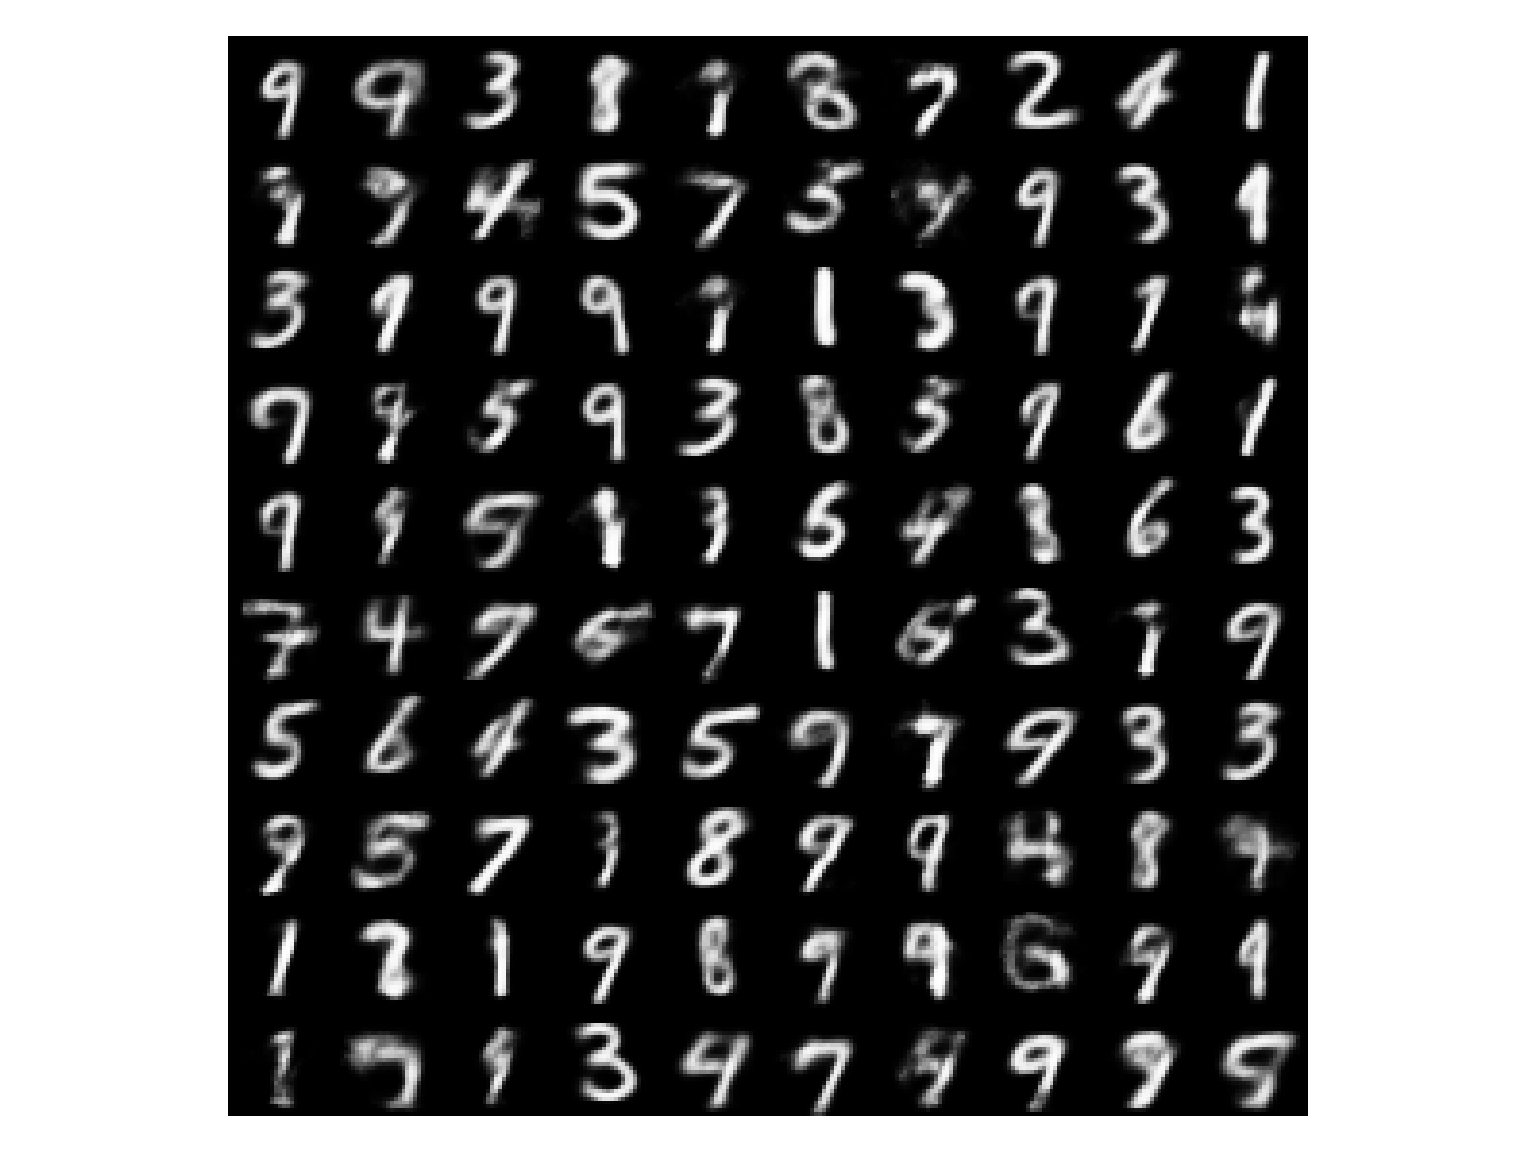
\includegraphics[height=200px]{includes/plots/gumbolt-vae/mnist/sampled.png}
		\caption{Sampling Plot for Gumbolt-Vae}
	\end{figure}
\end{frame}

\section{Stochastic Block Models}
\begin{frame}{Stochastic Block Models}
	A stochastic block model consists of
	\begin{itemize}
		\item A set of $N$ nodes/vertices, possibly with features $\set{\vx_{n}}$
		\item A partition of the nodes into $K$ communities $\set{\sC_k}$
		\item An adjacency matrix $\sA$ of link probabilities between nodes
	\end{itemize}

	Trained using EM algorithm, alternating between community structure (latent variables) and link likelihood parameters.
\end{frame}

\begin{frame}{Graph Variational Autoencoders}
	\bt{GCN:} Like a convolutional neural network, the features of a node and its neighbours are convoluted to compute inputs for the next layer

	\bt{GVAE}: A GCN is used to compute parameters for the latent representations (encoder), and the latent representaions are passed into a standard neural network to regenerate link probabilities (decoder).

	GVAEs use gaussian latent variables, and therefore the reparameterization is simple
\end{frame}

\begin{frame}{Graph Variational Autoencoders}

	\bt{Encoder:} Computes the means and log-variances of the latent variables using a GCN
	\begin{align*}
		\set{\mu_{n,k}, \sigma_{n,k}}_{k = 1}^K = \text{GCN}\para{\vx_n, \sA, \vphi}
	\end{align*}

	\bt{Decoder:} Generates edges/links (A) between nodes
	\begin{align*}
		\vz_n &\sim \ND{\vmu_n, \text{diag}(\vsigma_n^2)} \\
		A_{n,m} &\sim \sigma\para{\trans{\vf(\vz_n)} \vf(\vz_m)}
	\end{align*}

	Affords fast inference and excellent predictive power, however latent representations are non-interpretable

\end{frame}

\begin{frame}{Non-Parametric Latent Feature Relational Model}
	The latent features are binary vectors sampled using the Indian Buffet Process prior, and a weigh matrix sampled using a multivariate gaussian is used to compute link probabilities.
	\begin{align*}
		Z &\sim \text{IBP}(\alpha) \\
		w_{k,k'} &\sim \ND{0, \sigma^2} \\
		A_{n, m} &\sim \sigma(\trans{\vz_n} \sW \vz_m)
	\end{align*}

	This produces interpretable features, however it uses MCMC algorithm and, therefore, suffers from slow inference.
\end{frame}

\section{Gumbolt-VGAE}
\begin{frame}{Gumbolt Variational Graph Auto Encoder (Gumbolt-VGAE)}
	We try to combine the two approaches, \ie have interpretable latent representations along with a powerful predictive model. 

	Binary latent vectors ($\vb$) are used in company with real latent vectors ($\vr$), and the Gumbolt model (with RBM prior) is employed to reparameterize the binary latent vectors. Final latent representation $\vz$ is given as $\vz = \vb \odot \vr$
\end{frame}

\begin{frame}{Gumbolt-VGAE: VAE Encoder/Decoder}
	\bt{The Decoder}
	\begin{align*}
		\brac{\vb_1, \vb_2} \sim \text{RBM}\para{\va_1, \va_2, \sW}, \hspace{0.5cm} \vr \sim \ND{\vzero, \vI}
	\end{align*}
	\bt{The Encoder}
	\begin{align*}
		\qp{\vb_n, \vr_n \pipe \vx, \sA, \vphi} &= \prod_{k = 1}^K \qp{b_{n,k} \pipe \vx_n, \sA, \vphi} \qp{r_{n,k} \pipe \vx_n, \sA, \vphi}
	\end{align*}
	and
	\begin{align*}
		\qp{b_{n, k} \pipe \vx, \sA, \vphi} &= \text{Bernoulli}\para{\pi_{n, k}} \\
		\qp{r_{n, k} \pipe \vx, \sA, \vphi} &= \ND{\mu_{n, k}, \sigma_{n, k}^2}
	\end{align*}
	where $\set{\pi_{n, k}, \mu_{n, k}, \sigma_{n, k}}_{k = 1}^K= \text{GCN}(\vx_n, \sA)$.
\end{frame}

\begin{frame}{Results}
	\fontsize{7.5pt}{7.2}\selectfont
	\begin{table}
		\centering
		\begin{tabular}{l c c c c c c}
			\hline
			\bt{Method} & \quad & \multicolumn{2}{c}{\bt{Cora}} & \quad & \multicolumn{2}{c}{\bt{Citeseer}} \\
			\hline
			SC				& \quad & 0.8460 & 0.8850 & \quad & 0.8050 & 0.8500 \\
			DW				& \quad & 0.8310 & 0.8500 & \quad & 0.8050 & 0.8360 \\
			LFRM			& \quad & 0.9096 & 0.9060 & \quad & 0.8965 & 0.9118 \\
			VGAE			& \quad & 0.9260 & 0.9328 & \quad & 0.9200 & 0.9200 \\
			\hline
			Gumbolt-VGAE	& \quad & \bt{0.9282} & \bt{0.9396} & \quad & \bt{0.9230} & \bt{0.9339} \\
			\hline
		\end{tabular}
		\caption{Results (ROC and AP) of Gumbolt-VAE compared with baselines}
	\end{table}
\end{frame}

\end{document}
